%==========================
% Chapter 7: Diffusion and Score-Based Models
%==========================

\chapter{Diffusion and Score-Based Models}
\label{ch:diffusion_score}

\vspBlock

Transformers build probability distributions one token at a time, marching left to right through a sequence. Diffusion models take a completely different approach: they start with pure noise and gradually sculpt it into structured data, like a sculptor revealing a statue from marble. Instead of discrete steps through a vocabulary, diffusion operates in continuous space, progressively refining a sample through a series of denoising operations.

\vspPara

This chapter explores diffusion models through the lens of information geometry. We will see that adding noise is a controlled process of information destruction, and denoising is the reverse process of information recovery. The score function, which measures how probability density changes in space, becomes our guide through this space. Along the way, we will connect diffusion to variational inference, understand why different training objectives make different tradeoffs, and see how conditioning and guidance let us steer the generation process toward desired outcomes.

\vspChapter

The high-level symmetry between corruption and reconstruction is summarized in Figure~\ref{fig:forward_reverse}, which contrasts the forward destruction of information with the reverse trajectory that follows the learned score field.

\begin{figure}[t]
\centering
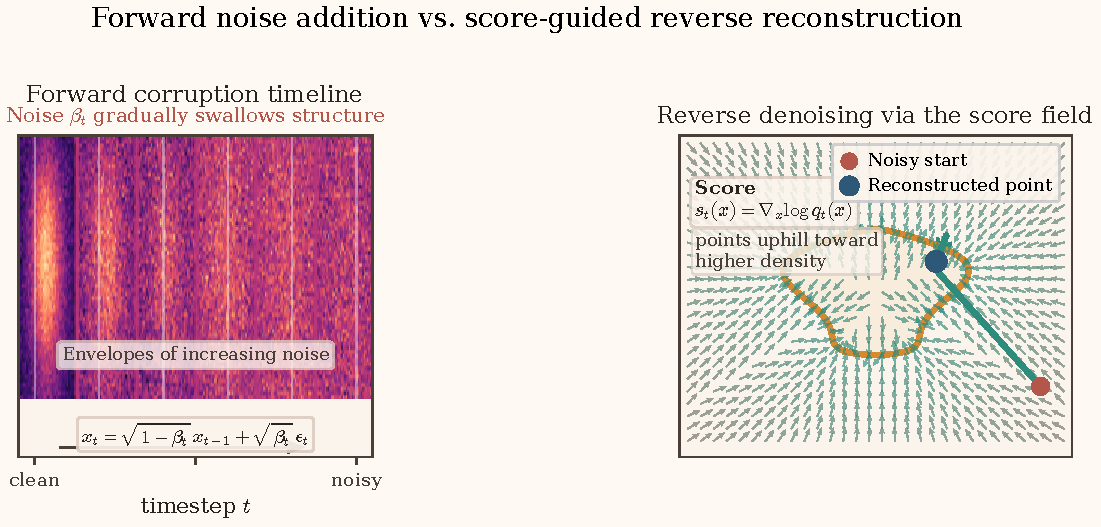
\includegraphics[width=\linewidth]{code/figures/ch07_diffusion_score/fig_7_1_forward_reverse.pdf}
\caption{The forward process slowly adds noise while the reverse process relies on the score to bring noisy samples back to the data manifold.}
\label{fig:forward_reverse}
\end{figure}

%==========================
\section{The Forward Process: Adding Noise as Information Destruction}

\vspSmall
\begin{keyinsight}
\textbf{Notation.} We use $q$ for the forward diffusion (data corruption) process and $p_\theta$ for the learned reverse process. $p_{\text{data}}$ is the true data distribution. Unless noted otherwise, $q_t(x)$ denotes the forward marginal of $x_t$ at time $t$ under $x_0\sim p_{\text{data}}$, and $s_t(x)=\nabla_x\log q_t(x)$ is its score. We write $q(x_t\mid x_0)$ for the closed-form Gaussian noising distribution and $q(x_{t-1}\mid x_t,x_0)$ for the corresponding posterior.
\end{keyinsight}

\label{sec:forward_process}
%==========================

\vspBlock

\subsection{From Data to Noise}

Imagine you have a crisp photograph. Now imagine gradually adding random noise to it: first a little grain, then more static, until eventually the image is completely unrecognizable, just pure white noise. This is the essence of the forward diffusion process.

\vspPara

Mathematically, we start with data $x_0$ drawn from some complex distribution $p_{\text{data}}(x_0)$, such as natural images or molecular structures. We then define a sequence of increasingly noisy versions $x_1, x_2, \ldots, x_T$ by repeatedly adding Gaussian noise:
%
\begin{equation}
x_t = \sqrt{1 - \beta_t} \, x_{t-1} + \sqrt{\beta_t} \, \epsilon_t
\end{equation}
%
where $\epsilon_t \sim \mathcal{N}(0, I)$ is standard Gaussian noise and $\beta_t \in (0,1)$ is a noise schedule that controls how much noise we add at step $t$.

\vspPara

It is convenient to define $\alpha_t = 1-\beta_t$ and the cumulative product $\bar{\alpha}_t = \prod_{s=1}^t \alpha_s$. With these, the $t$-step conditional distribution has the closed form
$$q(x_t\mid x_0)=\mathcal{N}\!\left(x_t;\sqrt{\bar{\alpha}_t}\,x_0, (1-\bar{\alpha}_t)I\right),$$
equivalently the reparameterization $x_t = \sqrt{\bar{\alpha}_t}\,x_0 + \sqrt{1-\bar{\alpha}_t}\,\epsilon$ with $\epsilon\sim\mathcal{N}(0,I)$. We will switch between $(\beta_t)$, $(\alpha_t)$, and $(\bar{\alpha}_t)$ notation as needed.
In other words, $q(x_t\mid x_0)$ is a simple Gaussian ``noising'' distribution whose mean shrinks the signal and whose variance grows with $t$.

\vspPara

The coefficient $\sqrt{1 - \beta_t}$ shrinks the previous signal, while $\sqrt{\beta_t}$ determines the amount of new noise. This particular form preserves unit variance when $x_{t-1}$ is standardized and independent of $\epsilon_t$: $\mathrm{Var}(x_t)=(1-\beta_t)\mathrm{Var}(x_{t-1})+\beta_t\mathrm{Var}(\epsilon_t)=1$. Over many steps, the signal $x_0$ becomes progressively weaker while the noise accumulates, until at time $T$, we have $x_T \approx \mathcal{N}(0, I)$, pure Gaussian noise.

\vspSection

\begin{keyinsight}
The forward process is a Markov chain that destroys information in a controlled way. Each step adds a calibrated amount of noise, gradually erasing the structure in the data until only randomness remains. Crucially, this process is designed so that we know the distribution of $x_t$ given $x_0$ in closed form, making it tractable to work with.
\end{keyinsight}

\vspSection


\subsection{Closed-Form Transition Kernel}

Because we are adding independent Gaussian noise at each step, we can write down the distribution of $x_t$ given $x_0$ without having to simulate all the intermediate steps. Define the cumulative noise level:
%
\begin{equation}
\bar{\alpha}_t = \prod_{s=1}^t (1 - \beta_s)
\end{equation}

\vspPara

\textbf{Why variance preservation matters.} Keeping $\mathrm{Var}(x_t)$ near 1 prevents numerical explosion/vanishing across many steps, makes the noise schedule interpretable, and ensures $x_T\approx\mathcal{N}(0,I)$ regardless of $x_0$ (so the terminal prior $p(x_T)$ is simple).

\vspPara

Then by repeated application of the transition kernel and using properties of Gaussian distributions, we get:
%
\begin{equation}
q(x_t \mid x_0) = \mathcal{N}(x_t; \sqrt{\bar{\alpha}_t} \, x_0, (1 - \bar{\alpha}_t) I)
\end{equation}

\vspPara

\textbf{Posterior of a single step.} The forward chain implies a Gaussian posterior
$$q(x_{t-1}\mid x_t,x_0)=\mathcal{N}\!\left(x_{t-1};\tilde{\mu}_t(x_t,x_0),\tilde{\beta}_t I\right),$$
with
$$\tilde{\mu}_t(x_t,x_0)=\frac{\sqrt{\bar{\alpha}_{t-1}}\,\beta_t}{1-\bar{\alpha}_t}x_0 + \frac{\sqrt{\alpha_t}(1-\bar{\alpha}_{t-1})}{1-\bar{\alpha}_t}x_t, \qquad \tilde{\beta}_t=\frac{1-\bar{\alpha}_{t-1}}{1-\bar{\alpha}_t}\,\beta_t.$$
This follows from standard Gaussian conditioning: multiply $q(x_t\mid x_{t-1})$ and $q(x_{t-1}\mid x_0)$ as functions of $x_{t-1}$ and complete the square. The closed form underpins the ELBO decomposition and practical samplers.

\vspPara

This says that $x_t$ is a noisy version of $x_0$, where the signal has been scaled by $\sqrt{\bar{\alpha}_t}$ and Gaussian noise with variance $(1 - \bar{\alpha}_t)$ has been added. As $t$ increases, $\bar{\alpha}_t$ decreases toward zero, so the signal component vanishes and the noise dominates.
\vspPara

The noise schedule $\{\beta_t\}$ is a design choice. Common choices include linear schedules ($\beta_t$ increases linearly from $\beta_1 \approx 10^{-4}$ to $\beta_T \approx 0.02$) and cosine schedules (which add noise more gradually at the beginning and end). The goal is to ensure that $x_T$ is close to pure noise while keeping each individual step $\beta_t$ small enough that local dynamics are smooth.

\vspSection

\begin{examplebox}
\textbf{Worked Example: Forward Diffusion in 1D}

Consider a simple 1D data distribution: a point mass at $x_0 = 5$. We apply forward diffusion with a constant noise schedule $\beta_t = 0.1$ for $T = 10$ steps.

After one step:
%
\begin{equation*}
\bar{\alpha}_1 = 1 - 0.1 = 0.9
\end{equation*}
%
so $x_1 \sim \mathcal{N}(5 \sqrt{0.9}, 0.1) \approx \mathcal{N}(4.74, 0.1)$.

After five steps:
%
\begin{equation*}
\bar{\alpha}_5 = 0.9^5 \approx 0.59
\end{equation*}
%
so $x_5 \sim \mathcal{N}(5 \sqrt{0.59}, 0.41) \approx \mathcal{N}(3.84, 0.41)$.

After ten steps:
%
\begin{equation*}
\bar{\alpha}_{10} = 0.9^{10} \approx 0.35
\end{equation*}
%
so $x_{10} \sim \mathcal{N}(5 \sqrt{0.35}, 0.65) \approx \mathcal{N}(2.96, 0.65)$.

The mean drifts toward zero and the variance increases, moving toward $\mathcal{N}(0,1)$ as $t \to \infty$.
\end{examplebox}

\vspSection

\subsection{Information-Theoretic View: Entropy Growth}

From an information perspective, the forward process increases entropy. The differential entropy of $x_t$ given $x_0$ is:
%
\begin{equation}
H(x_t \mid x_0) = \frac{d}{2} \log(2\pi e (1 - \bar{\alpha}_t))
\end{equation}
%
where $d$ is the dimensionality of $x$. As $\bar{\alpha}_t \to 0$, the entropy grows because the noise variance $(1 - \bar{\alpha}_t)$ increases toward 1.

\vspPara

The mutual information between $x_0$ and $x_t$ measures how much information about the original data remains after diffusion:
%
\begin{equation}
I(x_0; x_t) = H(x_t) - H(x_t \mid x_0)
\end{equation}

\vspPara

Because $x_0 \to x_t$ is a noisy Markov kernel, the data processing inequality tells us that $I(x_0; x_t)$ is nonincreasing in $t$: adding more noise cannot create information about the original data. (A small technical note: differential entropy depends on units and can be negative, so treat it as a geometric ``spread'' intuition rather than a literal bit count.)

\vspPara

This mutual information decreases as $t$ increases, quantifying the information destruction. At $t=0$, all information is preserved. At $t=T$, essentially no information remains: $x_T$ is indistinguishable from pure noise, regardless of what $x_0$ was.

\vspBlock

\begin{geometrylens}
Think of the forward process as a flow in probability space. We start with a complex, structured distribution $p_{\text{data}}(x_0)$ and flow toward the simple Gaussian $\mathcal{N}(0,I)$. At each step, the distribution spreads out and smooths, trading off structure for entropy. Geometrically, we are moving from a low-entropy, high-complexity region of the space of distributions toward a high-entropy, low-complexity attractor.
\end{geometrylens}

\vspChapter

%==========================
\section{The Reverse Process: Score Functions and Denoising}
\label{sec:reverse_process}
%==========================

\vspBlock

\subsection{Reversing the Noise: The Big Idea}

The forward process destroys information. The reverse process recovers it. If we can reverse the diffusion chain, starting from $x_T \sim \mathcal{N}(0,I)$ and working backward to $x_0$, we can generate samples from $p_{\text{data}}(x_0)$.

\vspPara

Here is the key insight: the reverse of a diffusion process is also a diffusion process, but run backward in time. However, reversing requires knowing something subtle: the score function, which tells us which direction to move in space to increase the probability density. To reverse diffusion, we must know which direction increases probability density---the score encodes precisely this direction.

\vspPara

The score function at time $t$ is defined as:
%
\begin{equation}
s_t(x) = \nabla_x \log q_t(x)
\end{equation}
%
where $q_t(x)$ is the marginal distribution of $x_t$ (averaging over all possible data points $x_0$). The score is a vector field that points in the direction of steepest increase of log-probability. If you are at a point $x$ in space, the score tells you which way to move to reach higher-density regions.

\vspSection

\begin{pausebox}
\textbf{Pause and Visualize.} Imagine a probability density as a surface with peaks and basins. The score function is like a compass that always points uphill, toward the nearest peak. If you stand in a basin and follow the score, you will move toward regions of high probability. In diffusion models, we use the score to guide noisy samples back toward the data manifold.
\end{pausebox}

\vspSection

\begin{pausebox}
\textbf{At a glance: training and sampling.}

\textbf{Training (noise prediction).}
\begin{enumerate}
\item Sample $x_0\sim p_{\text{data}}$, a time $t\sim\mathrm{Unif}\{1,\dots,T\}$, and noise $\epsilon\sim\mathcal{N}(0,I)$.
\item Form $x_t=\sqrt{\bar{\alpha}_t}\,x_0+\sqrt{1-\bar{\alpha}_t}\,\epsilon$.
\item Minimize $\lambda(t)\,\|\epsilon-\epsilon_\theta(x_t,t)\|^2$ (equivalently, match the score $s_\theta(x_t,t)=-\epsilon_\theta/\sqrt{1-\bar{\alpha}_t}$).
\end{enumerate}

\textbf{Sampling (ancestral DDPM).}
\begin{enumerate}
\item Sample $x_T\sim\mathcal{N}(0,I)$.
\item For $t=T,\dots,1$, use the network prediction (and optional guidance) to produce the mean/variance of $p_\theta(x_{t-1}\mid x_t)$, then sample $x_{t-1}$ (or take a deterministic step for DDIM / the probability flow ODE).
\end{enumerate}
\end{pausebox}

\vspSection

\vspPara
\textbf{Concrete reverse step (DDPM).} A common reverse transition is Gaussian:
$$p_\theta(x_{t-1}\mid x_t)=\mathcal{N}\!\left(x_{t-1};\mu_\theta(x_t,t),\sigma_t^2 I\right).$$
In the noise-prediction parameterization, one widely used mean is
$$\mu_\theta(x_t,t)=\frac{1}{\sqrt{\alpha_t}}\left(x_t-\frac{\beta_t}{\sqrt{1-\bar{\alpha}_t}}\,\epsilon_\theta(x_t,t)\right),$$
and we sample $x_{t-1}=\mu_\theta(x_t,t)+\sigma_t z$ with $z\sim\mathcal{N}(0,I)$. A common choice is $\sigma_t^2\in\{\beta_t,\tilde{\beta}_t\}$; setting $z=0$ yields a deterministic update (DDIM / probability-flow-style).

\subsection{Denoising as Score Estimation}

In practice, we do not have access to the true score $s_t(x)$ because we do not know the marginal distribution $q_t(x)$. Instead, we train a neural network $s_\theta(x,t)$ to approximate it. This is called score-based generative modeling.

\vspPara

The network takes as input a noisy sample $x_t$ and the time index $t$, and outputs an estimate of the score. During training, we generate pairs $(x_0, x_t)$ by sampling data and applying forward diffusion, then train the network on a computable score target at each noise level.
In denoising score matching, the supervised target is the \emph{conditional} score $\nabla_x \log q(x_t\mid x_0)$, which we can compute in closed form from the forward process. Averaged over $x_0\sim p_{\text{data}}$, the optimal predictor as a function of $(x_t,t)$ recovers the \emph{marginal} score $s_t(x)=\nabla_x\log q_t(x)$ that appears in the reverse-time dynamics.

\vspPara

Interestingly, predicting the conditional score is equivalent to predicting the noise. If $x_t = \sqrt{\bar{\alpha}_t} \, x_0 + \sqrt{1 - \bar{\alpha}_t} \, \epsilon$ where $\epsilon \sim \mathcal{N}(0,I)$, then:
%
\begin{equation}
\nabla_x \log q(x_t \mid x_0) = -\frac{\epsilon}{\sqrt{1 - \bar{\alpha}_t}}
\end{equation}

\vspPara

So learning the score is the same as learning to denoise: given $x_t$, predict the noise $\epsilon$ that was added. Up to a $t$-dependent scaling constant, predicting the conditional score and predicting the noise are equivalent. This connection makes training more intuitive: the model learns to undo the corruption introduced by the forward process.

\vspSection

\begin{examplebox}
\textbf{Worked Example: Score in 1D Gaussian Mixture}

Consider a mixture of two Gaussians in 1D:
%
\begin{equation*}
p(x) = \frac{1}{2} \mathcal{N}(x; -3, 1) + \frac{1}{2} \mathcal{N}(x; 3, 1)
\end{equation*}

The log-density is:
%
\begin{equation*}
\log p(x) = \log\left[ \frac{1}{2} e^{-(x+3)^2/2} + \frac{1}{2} e^{-(x-3)^2/2} \right] + \text{const}
\end{equation*}

The score is:
%
\begin{equation*}
s(x) = \frac{d}{dx} \log p(x) = \frac{-(x+3) e^{-(x+3)^2/2} - (x-3) e^{-(x-3)^2/2}}{e^{-(x+3)^2/2} + e^{-(x-3)^2/2}}
\end{equation*}

At $x = -3$, near the left mode, $s(-3) \approx 0$ because we are at a peak. At $x = 0$, the midpoint, $s(0) = 0$ by symmetry, but this is an unstable equilibrium. At $x = -5$ (far left), $s(-5) > 0$, pointing right toward the nearest mode.

The score function creates a vector field that pulls samples toward the two modes, making them attractors of the reverse diffusion process.
\end{examplebox}

\vspChapter

%==========================
\section{Score Matching and Training Objectives}
\label{sec:score_matching}
%==========================

\vspBlock

\subsection{The Score Matching Objective}

How do we train a network $s_\theta(x,t)$ to estimate the score? The naive approach would be to minimize:
%
\begin{equation}
\mathbb{E}_{t, x_t \sim q_t} \left[ \| s_\theta(x_t, t) - \nabla_x \log q_t(x_t) \|^2 \right]
\end{equation}

\vspPara

But this is circular: we do not know $\nabla_x \log q_t(x_t)$ because we do not know $q_t$. That is what we are trying to learn!

\vspPara

The solution is denoising score matching (DSM). Instead of matching the marginal score, we match the conditional score $\nabla_x \log q(x_t \mid x_0)$, which we can compute because we know the forward process. The DSM objective is:
%
\begin{equation}
\mathcal{L}_{\text{DSM}} = \mathbb{E}_{t, x_0 \sim p_{\text{data}}, x_t \sim q(\cdot \mid x_0)} \left[ \lambda(t) \| s_\theta(x_t, t) - \nabla_x \log q(x_t \mid x_0) \|^2 \right]
\end{equation}
%
where $\lambda(t)$ is a weighting function that balances different noise levels.

\vspPara

Because $q(x_t \mid x_0)$ is Gaussian, we know its score exactly:
%
\begin{equation}
\nabla_x \log q(x_t \mid x_0) = -\frac{x_t - \sqrt{\bar{\alpha}_t} \, x_0}{1 - \bar{\alpha}_t}
\end{equation}

\vspPara

Equivalently, since $x_t = \sqrt{\bar{\alpha}_t} \, x_0 + \sqrt{1 - \bar{\alpha}_t} \, \epsilon$, we can write:
%
\begin{equation}
\nabla_x \log q(x_t \mid x_0) = -\frac{\epsilon}{\sqrt{1 - \bar{\alpha}_t}}
\end{equation}

\vspPara

So the DSM objective becomes a noise prediction task: given $x_t$ and $t$, predict the noise $\epsilon$ that was added.

\vspSection

\begin{keyinsight}
Denoising score matching converts an intractable problem (estimating the score of an unknown distribution) into a tractable supervised learning problem (predicting noise given noisy data). The forward process generates unlimited training pairs, and the target is computable in closed form.
\end{keyinsight}

\vspSection


\vspPara
\textbf{Parameterizations.} In practice the network predicts either (i) noise $\epsilon_\theta(x_t,t)$, (ii) the clean $x_{0,\theta}(x_t,t)$, or (iii) a blend $v_\theta$; these are equivalent up to $t$-dependent transforms. The score can be recovered as $s_\theta(x_t,t)=-\epsilon_\theta/\sqrt{1-\bar{\alpha}_t}$.
\subsection{Connection to Denoising Autoencoders}

The DSM objective is closely related to training a denoising autoencoder. A denoising autoencoder takes a corrupted input $x_t$ and tries to reconstruct the clean input $x_0$. The loss is typically:
%
\begin{equation}
\mathcal{L}_{\text{DAE}} = \mathbb{E}_{x_0, x_t} \left[ \| f_\theta(x_t, t) - x_0 \|^2 \right]
\end{equation}

\vspPara

This looks different from DSM, but they are related. If we parameterize the network to predict the noise $\epsilon$ instead of $x_0$, the two objectives become equivalent (up to weighting). In practice, modern diffusion models often predict $\epsilon$ directly, making the connection explicit.

\vspPara

The key difference is philosophical: denoising autoencoders were originally motivated by representation learning, while score matching is motivated by density estimation and generative modeling. But the underlying math connects them: both are learning to reverse the corruption process.

\vspChapter

%==========================
\section{ELBO vs DSM: Different Information Tradeoffs}
\label{sec:elbo_vs_dsm}
%==========================

\vspBlock

\subsection{The ELBO Perspective}

Diffusion models can also be understood through the lens of variational inference. The goal is to maximize the log-likelihood of the data:
%
\begin{equation}
\log p_\theta(x_0) = \log \int p_\theta(x_{0:T}) \, dx_{1:T}
\end{equation}

\vspPara

This integral is intractable, so we introduce the forward process $q(x_{1:T} \mid x_0)$ as a variational distribution and derive the evidence lower bound (ELBO):
%
\begin{align}
\log p_\theta(x_0) &\geq \mathbb{E}_{q(x_{1:T} \mid x_0)} \left[ \log \frac{p_\theta(x_{0:T})}{q(x_{1:T} \mid x_0)} \right] \\
&= \mathbb{E}_q \left[ \log p_\theta(x_0 \mid x_1) \right] - \sum_{t=2}^T \mathbb{E}_{q(x_t\mid x_0)} \left[ D_{\text{KL}}(q(x_{t-1} \mid x_t, x_0) \| p_\theta(x_{t-1} \mid x_t)) \right] \\
&\quad - D_{\text{KL}}(q(x_T \mid x_0) \| p(x_T))
\end{align}
\vspPara
\textbf{Derivation (three steps).}

1) \emph{Basic ELBO.} Introduce the tractable forward process $q(x_{1:T}\mid x_0)$ and apply Jensen:
$$\log p_\theta(x_0) = \log \int \frac{p_\theta(x_{0:T})}{q(x_{1:T}\mid x_0)} q(x_{1:T}\mid x_0)\,dx_{1:T} \;\ge\; \mathbb{E}_q\Big[\log \tfrac{p_\theta(x_{0:T})}{q(x_{1:T}\mid x_0)}\Big].$$

2) \emph{Chain rules.} Factorize $p_\theta$ and $q$ using the Markov structure: $p_\theta(x_{0:T})=p(x_T)\prod_{t=1}^T p_\theta(x_{t-1}\mid x_t)$ and $q(x_{1:T}\mid x_0)=\prod_{t=1}^T q(x_t\mid x_{t-1})$.

3) \emph{Regroup.} Collect terms to obtain a reconstruction term $\mathbb{E}_q[\log p_\theta(x_0\mid x_1)]$, a sum of denoising KL terms $\sum_{t=2}^T \mathbb{E}_q\big[ D_{\mathrm{KL}}(q(x_{t-1}\mid x_t,x_0)\,\|\,p_\theta(x_{t-1}\mid x_t))\big]$, and a prior-matching term $D_{\mathrm{KL}}(q(x_T\mid x_0)\,\|\,p(x_T))$.

This exposes the learning problem as matching each \emph{reverse} step and the terminal prior.


\vspPara

This decomposition reveals the structure of the learning problem. The first term is a reconstruction term: how well can we reconstruct $x_0$ from $x_1$. The middle terms are denoising terms: at each step $t$, the model $p_\theta$ should match the posterior $q(x_{t-1} \mid x_t, x_0)$, which tells us how to denoise $x_t$ into $x_{t-1}$ given knowledge of the clean data $x_0$. The final term ensures that the endpoint $x_T$ matches the prior, which is just Gaussian noise.

\vspSection

\begin{geometrylens}
The ELBO view treats diffusion as a hierarchical latent variable model, where each $x_t$ is a latent variable encoding progressively coarser information about $x_0$. The KL terms measure the mismatch between the approximate posterior $p_\theta(x_{t-1} \mid x_t)$ and the true posterior $q(x_{t-1} \mid x_t, x_0)$ in probability space. Minimizing these reverse-KL terms is a KL projection onto the model family (an M-projection in Chapter~3's terminology): at each step, we choose the reverse transition in our parameterized family that is closest (in KL) to the true posterior induced by the forward process.
\end{geometrylens}

\vspSection

\subsection{DSM as an Alternative Objective}

The denoising score matching objective does not directly optimize the ELBO. Instead, it focuses on learning the score function at each noise level, which is sufficient for sampling via the reverse SDE.

\vspPara

So what is the relationship between ELBO and DSM? For the standard Gaussian reverse parameterization used in DDPMs, each ELBO denoising KL term reduces (up to constants) to a weighted squared error between a network prediction and a known target. In particular, if $p_\theta(x_{t-1}\mid x_t)$ is Gaussian with a fixed variance and a mean parameterized via noise prediction $\epsilon_\theta(x_t,t)$ (or equivalently $x_{0,\theta}$), then maximizing the ELBO is equivalent to minimizing a specific time-weighted MSE on $\epsilon_\theta$. DSM uses the same regression target but allows a user-chosen weighting $\lambda(t)$.

\vspPara

However, the weightings differ. The ELBO naturally weights different time steps according to their contribution to the log-likelihood, while DSM uses a weighting function $\lambda(t)$ that can be chosen for other reasons (such as numerical stability or sample quality).

\vspPara

This leads to a practical difference: models trained with DSM often produce better samples than those trained with the ELBO, even though the ELBO is the theoretically correct objective for likelihood maximization. Why? The ELBO emphasizes early time steps (small $t$, low noise) because those contribute most to the log-likelihood. But for sample quality, later time steps (high noise) matter more because they determine the global structure of the sample. DSM with uniform or slightly upweighted $\lambda(t)$ balances these concerns better.

\vspSection

\begin{pausebox}
\textbf{Pause and Reflect.} This is a recurring theme in generative modeling: the objective we optimize is not always perfectly aligned with what we care about. The ELBO maximizes likelihood, which is good for density estimation but may not prioritize perceptual quality. DSM optimizes score matching, which is more directly tied to the sampling process and often leads to better-looking generations. The choice of objective is an information-theoretic tradeoff between different notions of ``fit.''
\end{pausebox}

\vspSection


\vspBlock

\vspPara
\textbf{Why DSM can look better than ELBO in practice.} "Better" typically refers to perceptual quality (e.g., FID, human preference) rather than likelihood. ELBO aggregates per-step KLs with weights that emphasize small-noise steps, whereas a flat DSM loss treats times more uniformly. This shifts emphasis from fine-detail log-likelihood toward visually salient denoising. SNR-aware or clipped-SNR weightings often bridge the gap: they can yield crisp samples without overly penalizing high-noise steps.
\subsection{Choosing \texorpdfstring{$\lambda(t)$}{lambda(t)}: SNR Weighting and Sample Quality}
The DSM loss often includes a weight $\lambda(t)$. Two common choices are $\lambda(t)=1$ and $\lambda(t)=1/(1-\bar{\alpha}_t)$. The latter scales like the inverse noise variance and emphasizes low-noise (high-SNR) times, bringing DSM closer to ELBO weighting.

A useful lens is the \emph{signal-to-noise ratio} $\mathrm{SNR}(t)=\bar{\alpha}_t/(1-\bar{\alpha}_t)$. Weightings that upweight mid-SNR regions (or clip extremely small SNR, ``min-SNR'' heuristics) can improve perceptual quality at similar compute.

In practice, heavier emphasis on low-noise steps tends to improve sample fidelity (crisper details) but can slightly worsen likelihood estimates; flatter weights can improve coverage. Tune $\lambda(t)$ to match your goal.

\subsection{Continuous vs Discrete Time}


\vspPara
\textbf{Transition.} We now move from discrete steps $t=1,\dots,T$ to continuous time $t\in[0,T]$. The two views are equivalent in the small-step limit but differ in notation and solvers.

\begin{center}
\begin{tabular}{l|l|l}
\textbf{Aspect} & \textbf{Discrete (DDPM)} & \textbf{Continuous (SDE/ODE)} \\
\hline
Forward & $x_t=\sqrt{1-\beta_t}x_{t-1}+\sqrt{\beta_t}\,\epsilon_t$ & $dx= f(x,t)\,dt + g(t)\,dw$ \\
Training & noise-prediction / score-matching & score-matching over $t\in[0,T]$ \\
Reverse & Markov chain $p_\theta(x_{t-1}\mid x_t)$ & reverse SDE or probability-flow ODE \\
Sampling & ancestral steps; DDIM & SDE solvers; ODE solvers (deterministic) \\
\end{tabular}
\end{center}
Here $w$ is a standard Wiener process (Brownian motion). Many score-based SDE models use a variance-preserving (VP) forward SDE, for example $dx=-\tfrac{1}{2}\beta(t)\,x\,dt+\sqrt{\beta(t)}\,dw$, whose small-step discretization resembles the DDPM update above.
\vspPara
\textbf{Reverse-time SDE (VP case).} Running the VP SDE backward from $T$ to $0$ yields a reverse-time dynamics whose drift is corrected by the score:
$$dx=\Big(-\tfrac{1}{2}\beta(t)\,x-\beta(t)\,s_t(x)\Big)dt+\sqrt{\beta(t)}\,d\bar{w},$$
where $\bar{w}$ is a Brownian motion when time runs backward. This is the sense in which learning $s_t$ is enough to generate samples: it fills in the missing piece of the reverse drift.
So far, we have discussed diffusion in both discrete time (steps $t = 1, 2, \ldots, T$) and continuous time (SDE with $t \in [0,T]$). These are not just notational differences; they represent different modeling choices with different tradeoffs.

\vspPara

\textbf{Discrete-time diffusion models} (like DDPM, the Denoising Diffusion Probabilistic Model) use a fixed number of steps $T$ (often 1000) and typically train a single time-conditioned denoising network shared across all steps. The ELBO can be written as a sum of KL divergences across timesteps. Sampling requires iterating through many steps, which is slow.

\vspPara

\textbf{Continuous-time diffusion models} (like score-based SDEs) treat time as continuous and train a single network $s_\theta(x,t)$ that takes $t$ as an input. The SDE perspective allows flexible sampling strategies: we can use fewer steps by discretizing the SDE more coarsely, or even use deterministic ODE solvers (via the probability flow ODE), trading off stochasticity for speed.

\vspPara

The continuous-time view also unifies diffusion with other models. For example, the probability flow ODE, which is the deterministic version of the reverse SDE, can be connected to neural ODEs and normalizing flows, revealing deep relationships between these model families.

\vspChapter

%==========================
\section{Guidance, Conditioning, and Classifier-Free Tricks}
\label{sec:guidance}
%==========================

\vspBlock

\subsection{Conditional Generation: The Challenge}

Often, we do not just want to generate samples from $p_{\text{data}}(x)$; we want to generate samples conditioned on some information $y$. For example, $y$ might be a text prompt (``a photo of a cat'') and $x$ might be an image. The goal is to sample from $p(x \mid y)$.

\vspPara

The naive approach is to train a conditional diffusion model $p_\theta(x_{t-1} \mid x_t, y)$ by simply feeding $y$ as an additional input to the denoising network. This works, but it has a problem: the model may not pay enough attention to the conditioning information. If $y$ provides only weak guidance, the generated samples may largely ignore it.

\vspPara

Guidance is a technique to amplify the effect of the conditioning, making the samples more strongly aligned with $y$. There are two main approaches: classifier guidance and classifier-free guidance.

\vspSection

\subsection{Classifier Guidance}

Classifier guidance uses an auxiliary classifier $p_\phi(y \mid x_t, t)$ that predicts the label $y$ from a noisy sample $x_t$. The idea is to modify the reverse diffusion process to favor samples that the classifier is confident about.

\vspPara

Using Bayes' rule, we can write the conditional score as:
%
\begin{align}
\nabla_x \log p(x_t \mid y) &= \nabla_x \log q_t(x_t) + \nabla_x \log p(y \mid x_t) \\
&= s_t(x_t) + \nabla_x \log p_\phi(y \mid x_t, t)
\end{align}

\vspPara

The conditional score is the unconditional score plus a gradient from the classifier. This gradient term pushes $x_t$ in the direction that increases the probability of $y$ according to the classifier.

\vspPara

We can strengthen this effect by introducing a guidance scale $w > 1$:
%
\begin{equation}
\tilde{s}_t(x_t, y) = s_t(x_t) + w \, \nabla_x \log p_\phi(y \mid x_t, t)
\end{equation}

\vspPara

When $w = 1$, we recover the true conditional score. When $w > 1$, we amplify the classifier's influence, making the samples more strongly conditioned on $y$ at the cost of some diversity (since we are moving away from the true posterior).

\vspSection

\begin{keyinsight}
Classifier guidance trades off between sample diversity and conditioning strength. Higher $w$ produces samples that better match the conditioning $y$ but are less diverse and may be less realistic. This is a bias-variance tradeoff: we bias the generation toward $y$ and reduce the variance of the conditional distribution.
\end{keyinsight}

\vspSection

\subsection{Classifier-Free Guidance}

Classifier guidance requires training a separate classifier $p_\phi(y \mid x_t, t)$, which is expensive and adds complexity. Classifier-free guidance achieves similar effects without an auxiliary model.

\vspPara

The idea is to train a single conditional model $s_\theta(x_t, t, y)$ but also enable unconditional generation by sometimes training with $y$ set to a null token (e.g., $y = \emptyset$). This creates a model that can estimate both the conditional score $s_\theta(x_t, t, y)$ and the unconditional score $s_\theta(x_t, t, \emptyset)$.

\vspPara

At sampling time, we interpolate between these two scores:
%
\begin{equation}
\tilde{s}_t(x_t, y) = s_\theta(x_t, t, \emptyset) + w \left( s_\theta(x_t, t, y) - s_\theta(x_t, t, \emptyset) \right)
\end{equation}

\vspPara

When $w = 0$, we get the unconditional score. When $w = 1$, we get the conditional score. When $w > 1$, we extrapolate beyond the conditional score, amplifying the effect of $y$.

\vspPara

Why does this work? The term $s_\theta(x_t, t, y) - s_\theta(x_t, t, \emptyset)$ is the gradient of $\log p(y \mid x_t)$ by Bayes' rule. So classifier-free guidance implicitly uses the model's own implicit classifier, avoiding the need for an external one.

\vspSection

\begin{examplebox}
\textbf{Worked Example: Text-to-Image with Classifier-Free Guidance}

Suppose we are generating an image conditioned on the text prompt $y = $ ``a red apple.'' We train a diffusion model that takes both $x_t$ and $y$ as input, with 10\% of training examples using $y = \emptyset$ (no prompt).

At sampling time, we start with $x_T \sim \mathcal{N}(0, I)$ and run the reverse process with guidance scale $w = 7$. At each step, we compute:
%
\begin{align*}
s_{\text{uncond}} &= s_\theta(x_t, t, \emptyset) \\
s_{\text{cond}} &= s_\theta(x_t, t, \text{``a red apple''}) \\
\tilde{s} &= s_{\text{uncond}} + 7 (s_{\text{cond}} - s_{\text{uncond}})
\end{align*}

The amplified score $\tilde{s}$ pushes the sample strongly toward images of red apples. With $w = 1$, we get realistic but sometimes loosely-related images. With $w = 7$, we get highly-aligned images that clearly depict red apples, though they may be slightly less diverse or more stylized.
\end{examplebox}

\vspPara
Figure~\ref{fig:guidance_interpolation} illustrates three guidance settings (unconditional, conditional, and guided) as $w$ grows.

\begin{figure}[t]
\centering
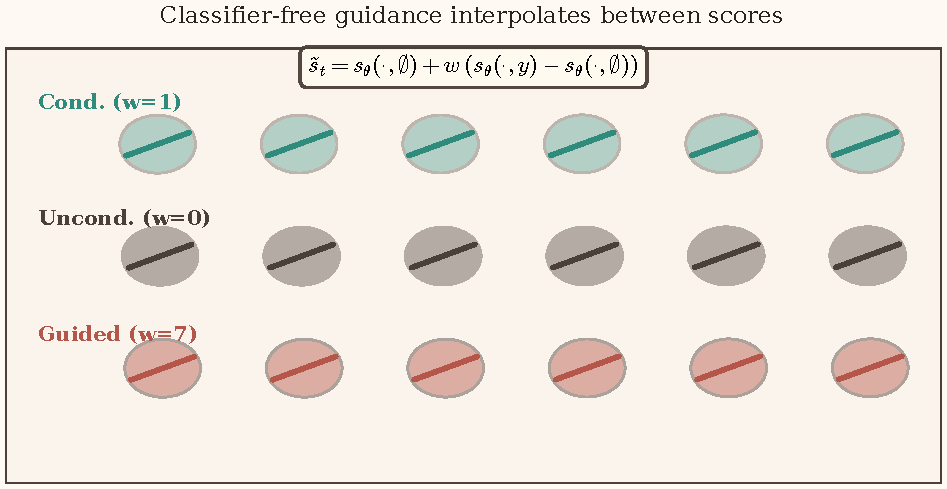
\includegraphics[width=\linewidth]{code/figures/ch07_diffusion_score/fig_7_5_guidance.pdf}
\caption{Classifier-free guidance blends unconditional and conditional score estimates, letting $w$ control how far to push past the unconditional gradient.}
\label{fig:guidance_interpolation}
\end{figure}

\vspChapter

%==========================

\subsection{Pitfalls of Guidance}
Increasing guidance weight $w$ strengthens conditioning but can oversaturate colors/textures, reduce diversity, and bias the sampler toward a narrow subset of modes. There is no universal $w$; tune per task/dataset, and watch for mode collapse and artifacts at high $w$. Classifier-free guidance also shifts the effective score scale, which may require retuning step size or noise schedule at sampling time.
\section{Geometry of Denoising Fields}
\label{sec:geometry_denoising}
%==========================

\vspBlock

\subsection{Score as a Vector Field}

The score function $s_t(x) = \nabla_x \log q_t(x)$ is a vector field on the data space. At each point $x$ and time $t$, it assigns a vector pointing in the direction of increasing log-probability density.

\vspPara

We can visualize this field in low dimensions. For a 2D distribution, the score function creates a field of arrows, with longer arrows in low-density regions (where the gradient is steep) and shorter arrows near mode centers (where the gradient is flat).

\vspPara

The reverse diffusion process follows these arrows. Starting from a random point in $x_T \sim \mathcal{N}(0,I)$, we move along the (learned) score field toward higher-density regions. The stochastic term can help exploration and reduce sensitivity to local score errors, but it does not guarantee avoidance of poor modes; the behavior depends on discretization, step sizes, and score accuracy. Ideally, trajectories end near high-density regions of $q_0(x)=p_{\text{data}}(x)$.

\vspPara
Figure~\ref{fig:score_vector_field} visualizes this intuition with a 2D score field and nominal reverse trajectory that climbs toward the nearest mode.

\vspSection

\begin{geometrylens}
The score field defines a gradient-flow-like structure on the manifold of probability distributions. Each integral curve of the field represents a trajectory from noise to data. The reverse SDE combines a drift aligned with the score with an injected noise term; heuristically this resembles stochastic gradient ascent, and the stochasticity can help exploration. The geometry of this field encodes the structure of the data distribution: modes become attractors, valleys become basins, and saddle points become decision boundaries.
\end{geometrylens}

\vspSection


\begin{figure}[t]
\centering
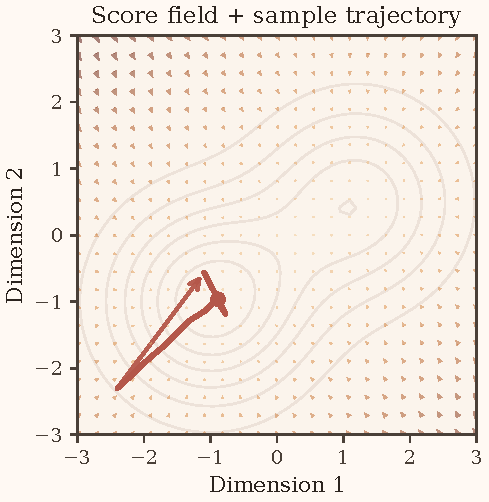
\includegraphics[width=\linewidth]{code/figures/ch07_diffusion_score/fig_7_2_score_field.pdf}
\caption{2D score vector field: arrows point toward higher probability density; reverse diffusion trajectories follow the field back to data modes (contours), with color indicating score magnitude.}
\label{fig:score_vector_field}
\end{figure}
\subsection{Tweedie's Formula and Conditional Expectations}

There is a beautiful connection between the score function and conditional expectations, known as Tweedie's formula. For a Gaussian observation model, the posterior mean of the clean signal given a noisy observation is:
%
\begin{equation}
\mathbb{E}[x_0 \mid x_t] = \frac{1}{\sqrt{\bar{\alpha}_t}}\left(x_t + (1 - \bar{\alpha}_t) \nabla_x \log q_t(x_t)\right)
\end{equation}
\vspPara
\textbf{Two-line sketch.} For $y=x+\eta$ with $\eta\sim\mathcal{N}(0,\sigma^2 I)$, Stein's identity (an integration-by-parts identity for Gaussian noise) gives $\nabla_y\log p(y)=\frac{\mathbb{E}[x\mid y]-y}{\sigma^2}$. Rearrange to get $\mathbb{E}[x\mid y]= y + \sigma^2\nabla_y\log p(y)$. Here $x=\sqrt{\bar{\alpha}_t}\,x_0$, $y=x_t$, and $\sigma^2=1-\bar{\alpha}_t$, so divide by $\sqrt{\bar{\alpha}_t}$ to recover $\mathbb{E}[x_0\mid x_t]$.


\vspPara

This says that the score function tells us how to adjust the noisy observation $x_t$ to get the best estimate (in the mean-squared-error sense) of the clean data $x_0$. The adjustment is proportional to the score, scaled by the noise variance.

\vspPara

Tweedie's formula gives us an alternative interpretation of the denoising process: each step of reverse diffusion is implicitly estimating the clean data, then adding noise to move toward the next step. The score function is the optimal bias correction that accounts for the fact that $x_t$ is not the true data but a noisy sample.

\vspSection

\begin{figure}[t]
\centering
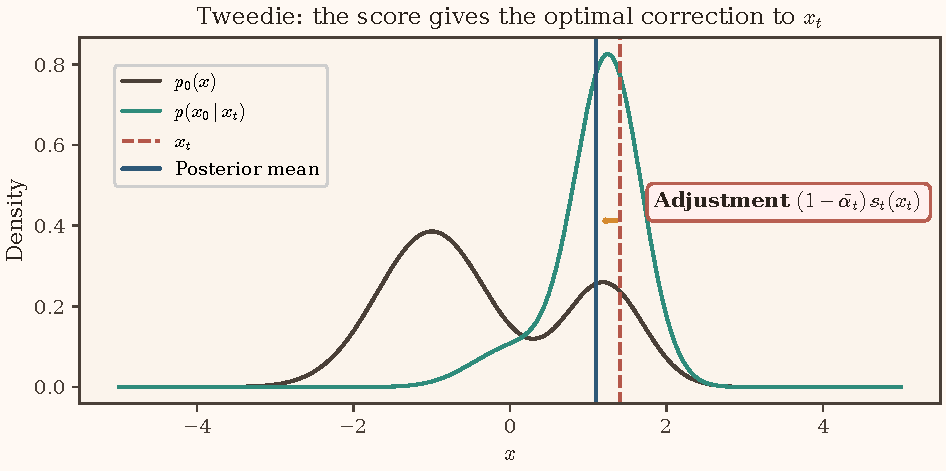
\includegraphics[width=\linewidth]{code/figures/ch07_diffusion_score/fig_7_4_tweedie.pdf}
\caption{Tweedie's formula: the score tells us how much to shift $x_t$ to recover the posterior mean of $x_0$.}
\label{fig:tweedie_formula}
\end{figure}

\vspSection

\subsection{Multi-Scale Denoising}

One of the key insights from diffusion models is that different noise levels correspond to different scales of structure. At high noise levels (large $t$), the score function captures coarse, global features: the overall shape, the primary modes, the broad layout. At low noise levels (small $t$), the score captures fine details: textures, edges, high-frequency content.

\vspPara

This multi-scale structure is why the DSM objective trains on all noise levels: the model needs to learn both coarse and fine denoising. If we only trained at low noise, the model would not learn the global structure. If we only trained at high noise, the model would not learn the details.

\vspPara

This is also why the noise schedule matters. A good schedule ensures that the model sees a balanced range of noise levels during training, from nearly clean data to nearly pure noise, so it learns the full spectrum of scales.

\vspSection

\vspPara
Figure~\ref{fig:noise_schedule} tracks a realistic noise schedule and its implied SNR, highlighting which timesteps emphasize coarse versus fine structure.

\begin{figure}[t]
\centering
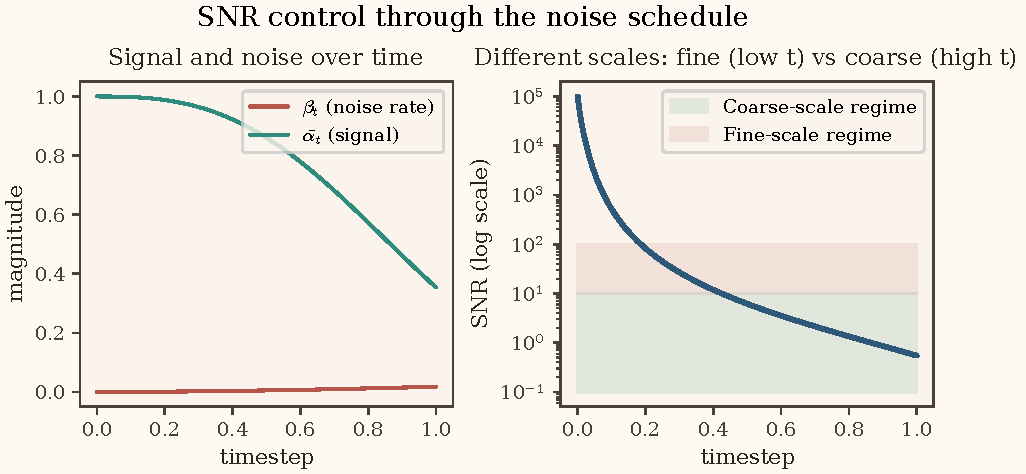
\includegraphics[width=\linewidth]{code/figures/ch07_diffusion_score/fig_7_3_noise_schedule.pdf}
\caption{Noise schedule, signal retention, and the resulting SNR, showing how the model sees finer textures at low $t$ (high SNR) and coarser patterns at high $t$ (low SNR).}
\label{fig:noise_schedule}
\end{figure}

\vspSection

\begin{pausebox}
\textbf{Pause and Connect.} Think about how this differs from autoregressive models like transformers. Transformers build sequences token by token, each step refining the entire sequence. Diffusion models build samples scale by scale, each step refining all pixels simultaneously but at different frequencies. Neither is inherently better; they are complementary approaches suited to different types of data and structure.
\end{pausebox}

\vspChapter

%==========================
\section{Connections to Other Models}
\label{sec:connections}
%==========================

\vspBlock

\subsection{VAEs and the ELBO Connection}

Diffusion models are closely related to variational autoencoders (VAEs), which we will explore in depth in Chapter 8. Both use latent variables and optimize an ELBO. The key difference is the structure of the latent space.

\vspPara

In a VAE, there is typically a single latent variable $z$ with low dimension compared to $x$. The latent space is a compressed representation learned by the encoder.

\vspPara

In a diffusion model, the ``latent variables'' are $x_1, \ldots, x_T$, which have the same dimension as $x_0$. The latent space is not compressed but progressively noised. Each $x_t$ is a different noise level of the same data, rather than a semantic encoding.

\vspPara

This difference has implications. VAEs are good at learning disentangled representations and performing interpolation in latent space. Diffusion models are good at generating high-quality samples and modeling fine details. The ELBO perspective reveals that both are doing variational inference, but with different architectural priors about what the latents should look like.

\vspSection

\subsection{Normalizing Flows and Deterministic Paths}

Normalizing flows (also in Chapter 8) are another family of generative models that transform a simple base distribution into a complex data distribution via a sequence of invertible transformations.

\vspPara

Diffusion models can be connected to flows through the \emph{probability flow ODE} (next subsection). Integrating this deterministic dynamics maps $x_T$ to $x_0$; under mild regularity, the resulting flow map is invertible and can in principle support likelihood evaluation via the instantaneous change-of-variables formula.

\vspPara

The difference is that diffusion models learn the score/velocity field via denoising, while normalizing flows explicitly parameterize the invertible map as a composition of invertible layers. Diffusion models are more flexible because they do not require invertibility during training, but flows have the advantage that sampling and likelihood are exact given the learned map.

\vspSection


\vspLarge
\subsection{Probability Flow ODE}
The probability flow ODE is a deterministic dynamics constructed to share the same marginal distributions as the corresponding diffusion SDE (see Song et al.\ (2021) for a derivation via the Fokker--Planck equation). For the variance-preserving (VP) case:
$$\frac{dx}{dt} = -\tfrac{1}{2}\beta(t)\,x - \tfrac{1}{2}\beta(t)\,s_t(x).$$
This connects diffusion to continuous normalizing flows: one can sample deterministically with high-order ODE solvers and, with a divergence/trace estimator plus numerical care, evaluate likelihoods via the instantaneous change-of-variables formula.

\subsection{Langevin Dynamics and MCMC}

The reverse SDE is a form of Langevin dynamics, a classical method for sampling from a distribution using gradient information. Langevin dynamics iterates:
%
\begin{equation}
x_{k+1} = x_k + \frac{\delta}{2} \nabla_x \log p(x_k) + \sqrt{\delta} \, \eta_k
\end{equation}
%
where $\eta_k \sim \mathcal{N}(0,I)$ is noise and $\delta>0$ is a step size.

\vspPara

This looks similar to the reverse SDE discretization. The difference is that Langevin dynamics assumes we have the score of the target distribution $p(x_0)$, while diffusion models learn a sequence of scores for the noised distributions $q_t(x_t)$. By starting from pure noise and gradually denoising, diffusion models sidestep some of the mixing-time issues that plague Langevin MCMC on complex distributions.

\vspPara

This connection suggests that diffusion models can be viewed as ``annealed Langevin dynamics,'' where we start from an easy distribution (Gaussian noise) and gradually anneal toward the target distribution, using the score at each noise level as a guide.

\vspChapter

%==========================
\section{Practical Considerations and Extensions}

\vspLarge
\subsection{Architectures: U-Nets, Time Embeddings, and Attention}
Most image diffusion models use U-Net backbones with residual blocks, skip connections, and attention at multiple scales. Time is encoded via sinusoidal/Fourier features and injected with MLPs into normalization layers. Conditional models add cross-attention (e.g., on text or layout) in higher-resolution blocks. GroupNorm (or LayerNorm in latent models) stabilizes training.

\vspMed
\subsection{Training Tricks and Schedules}
Exponential moving average (EMA) of weights improves sample quality. Cosine/linear LR schedules with warmup are common; gradient clipping helps stability. Batch sizes depend on resolution; accumulate gradients if needed. Mix $t$ uniformly or SNR-aware; match $\lambda(t)$ to your sampling targets.

\vspMed
\subsection{Debugging and Diagnostics}
Sanity checks: verify the forward noising code, plot $\|\epsilon_\theta(x_t,t)\|^2$ vs. $t$, and confirm denoising works on synthetic Gaussians. Early failures include blurry reconstructions (under-emphasis on low-noise steps), training divergence (LR too high), and mis-scaled time embeddings.
\label{sec:practical}
%==========================

\vspBlock

\subsection{Sampling Speed: The Iteration Bottleneck}

One of the main criticisms of diffusion models is that sampling is slow. We need to simulate hundreds or thousands of diffusion steps to generate a single sample, and each step requires a neural network evaluation.

\vspPara

There are several approaches to speed up sampling:

\vspPara

\textbf{Fewer steps with better discretization.} Instead of using 1000 steps, use 50 steps with a carefully chosen discretization of the SDE. DDIM (Denoising Diffusion Implicit Models) is one such method that uses a deterministic update rule allowing larger steps.

\vspPara

\textbf{Distillation.} Train a separate model to predict multiple steps of the diffusion process at once, effectively ``compressing'' the trajectory. Progressive distillation can reduce the number of steps from 1000 to 4 with minimal quality loss.

\vspPara

\textbf{Consistency models.} Learn a function that directly maps any noisy $x_t$ to the clean $x_0$, allowing one-step generation. This requires a different training procedure but can achieve comparable quality with far fewer evaluations.

\vspSection

Figure~\ref{fig:sampling_speed} summarises the quality-vs-compute tradeoff for each sampler. We measure compute via NFE (number of function evaluations / network calls) and quality via FID (Fr\'echet Inception Distance; lower is better), then break total wall-clock time into the dominant overheads.

\begin{figure}[t]
\centering
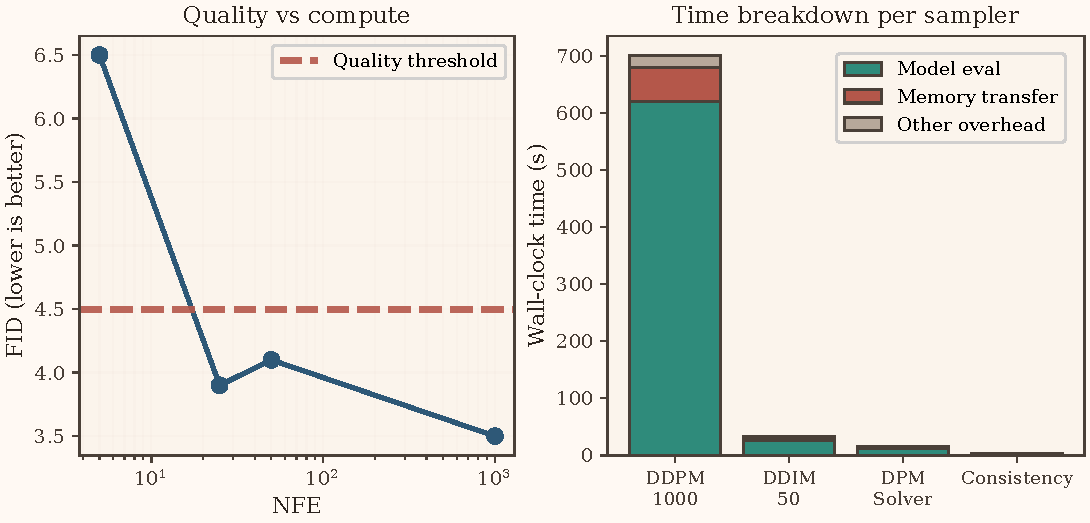
\includegraphics[width=\linewidth]{code/figures/ch07_diffusion_score/fig_7_6_sampling_speed.pdf}
\caption{Left: log-$x$ plot of NFE vs.\ FID for different samplers. Right: stacked wall-clock time per method, illustrating where the cost is incurred.}
\label{fig:sampling_speed}
\end{figure}

\vspLarge
\subsection{Algorithmic Families for Fast Sampling}
\textbf{Ancestral (DDPM).} Stochastic, many steps, stable.

\textbf{DDIM.} Deterministic or partially stochastic non-Markovian updates; preserves a fixed noise path; fewer steps at similar quality.

\textbf{Higher-order solvers (e.g., DPM-Solver).} Treat the reverse dynamics as an ODE/SDE and apply tailored exponential integrators to reduce the number of function evaluations (NFE) while preserving quality.

Quality typically improves with NFE, but good solvers close the gap quickly; report both NFE and metrics when comparing methods.
\subsection{Continuous-Time and Variance Reduction}

Training diffusion models in continuous time with the score matching objective can suffer from high variance in gradient estimates, especially at high noise levels where the score magnitude is large.

\vspPara

Variance reduction techniques include:

\vspPara

\textbf{Importance sampling over time.} Instead of uniformly sampling $t$, sample more frequently from noise levels where the gradient has higher magnitude, then reweight the loss.

\vspPara

\textbf{Score weighting.} Use a weighting function $\lambda(t)$ in the DSM objective that downweights high-noise levels, where score estimation is noisier.

\vspPara

\textbf{Exponential moving average (EMA).} Maintain an EMA of the model weights during training and use the EMA model for sampling. This smooths out high-frequency oscillations in the learned score function.

\vspSection

\subsection{Latent Diffusion Models}

Diffusion models work well on high-dimensional data like images, but the computational cost scales with dimension. For very large images (e.g., 1024x1024), running diffusion in pixel space becomes prohibitively expensive.

\vspPara

Latent diffusion models solve this by first training an autoencoder (typically a VAE) to compress images into a lower-dimensional latent space, then running diffusion in this latent space. The denoising network operates on latent codes rather than pixels, reducing memory and compute requirements.

\vspPara

Stable Diffusion, one of the most popular text-to-image models, is a latent diffusion model. It combines a VAE for compression, a U-Net for denoising, and a text encoder (like CLIP) for conditioning. By working in latent space, it achieves high quality while being efficient enough to run on consumer GPUs.

\vspChapter

%==========================

\vspLarge
\subsection{Alternative Degradations (``Cold Diffusion'')}
Diffusion need not use Gaussian noise. One can diffuse with blurring, masking/inpainting operators, or other corruptions, provided the reverse dynamics are learnable. Such choices tailor the inductive bias to the task (e.g., super-resolution with blur kernels). They typically require re-deriving the training target to match the corruption.

\vspChapter

\section{Looking Forward}
\label{sec:looking_forward}
%==========================

\vspBlock

Diffusion models have rapidly become a dominant paradigm for generative modeling, rivaling and often surpassing GANs and VAEs in sample quality. They have also expanded beyond images to audio, video, 3D shapes, molecular structures, and even discrete data like text.

\vspPara

From an information-geometric perspective, diffusion models are elegant: they transform a complex distribution into a simple one via a series of small steps, each guided by the local geometry of the score function. The reverse process is the corresponding reverse-time dynamics of the forward process, recovering information that was systematically destroyed.

\vspPara

In the next chapter, we will explore VAEs and normalizing flows in greater depth, seeing how these models relate to diffusion through the lens of the ELBO and change-of-variables. We will also discuss how all three model families---autoregressive, diffusion-based, and flow-based---make different tradeoffs between sample quality, likelihood estimation, and computational efficiency. The unifying thread is information geometry: each model defines a trajectory through the space of distributions, and understanding these trajectories helps us design better models and choose the right tool for each task.

\vspBlock

\begin{pausebox}
\textbf{Chapter Summary.} Diffusion models generate samples by reversing a process that gradually adds noise to data. The forward process destroys information in a controlled way, transforming structured data into Gaussian noise. The reverse process recovers information by following the score function, which points toward high-probability regions. We can train these models using denoising score matching, which learns to predict noise at each noise level. Guidance techniques let us condition generation on additional information, trading off between diversity and alignment. Diffusion connects to VAEs through the ELBO, to flows through deterministic ODEs, and to Langevin dynamics through stochastic gradient flows.
\end{pausebox}

\vspSection

\begin{pausebox}
\textbf{Further Reading.} Good entry points to the diffusion/score literature:
\begin{itemize}
\item Ho et al. (2020): \emph{Denoising Diffusion Probabilistic Models (DDPM)}.
\item Song, Meng \& Ermon (2020): \emph{Denoising Diffusion Implicit Models (DDIM)}.
\item Song et al. (2021): \emph{Score-Based Generative Modeling through Stochastic Differential Equations}.
\item Nichol \& Dhariwal (2021): \emph{Improved DDPM} (noise schedules, likelihood improvements).
\item Dhariwal \& Nichol (2021): \emph{Diffusion Models Beat GANs on Image Synthesis} (guidance, scaling).
\item Ho \& Salimans (2022): \emph{Classifier-Free Diffusion Guidance}.
\item Lu et al. (2022): \emph{DPM-Solver} (fast ODE/SDE solvers for sampling).
\item Rombach et al. (2022): \emph{High-Resolution Image Synthesis with Latent Diffusion Models}.
\end{itemize}
\end{pausebox}

\vspSection

\section*{Exercises}
\begin{enumerate}
\item Derive $q(x_t\mid x_0)$ for the variance-preserving chain with $\alpha_t=1-\beta_t$.
\item Show that the DSM objective with $\lambda(t)=1$ differs from ELBO weighting and relate both to SNR.
\item Prove the closed form of $q(x_{t-1}\mid x_t,x_0)$ and identify $\tilde{\mu}_t,\tilde{\beta}_t$.
\item Starting from the reverse SDE, derive the probability flow ODE.
\item Implement ancestral DDPM sampling; measure quality vs. number of function evaluations (NFE).
\item Implement DDIM sampling and compare with DDPM at the same NFE.
\item Verify Tweedie's formula numerically on a synthetic 2D mixture of Gaussians.
\item Explore guidance: plot a metric of diversity vs. guidance scale $w$ on a conditional task.
\item (Hard) Train a tiny UNet on MNIST with min-SNR weighting; compare sample quality to uniform weighting.
\end{enumerate}

\vspChapter
